\section{Combinaison de classifieurs}

\subsection{Combinaison par somme et produit de probabilités}

Même si le second classifieur affiche un taux de reconnaissance plus élevé que le premier, on peut imaginer que les résultats obtenus puissent être complémentaires. C'est pourquoi, afin d'améliorer le taux de reconnaissance global du système, il est possible de combiner les probabilités obtenues par chaque classifieur afin d'obtenir un nouveau vecteur de probabilité d'appartenance. On espère le résultat ainsi obtenu plus précis que ceux donnés par leur utilisation indépendante,.\\
Deux méthodes de combinaison sont utilisées : la somme et le produit.\\
Soient pbelonging1 et pbelonging2 les probabilités d'appartenance respectivement obtenus pour les classifieurs 1 et 2. Les nouvelles probabilités, obtenues par combinaison en utilisant la somme et le produit, sont données de la façon suivante :

$$\begin{array}{rcl}
pbelongingsum(x/\omega_i) &=& pbelonging1(x/\omega_i) + pbelonging2(x/\omega_i)\\
pbelongingprod(x/\omega_i) &=& pbelonging1(x/\omega_i)pbelonging2(x/\omega_i)
\end{array}$$

avec $x$ l'objet testé pour la classe d'appartenance $\omega_i$


\subsection{Critique des résultats obtenus}

\begin{figure}[h]
	\begin{center}
		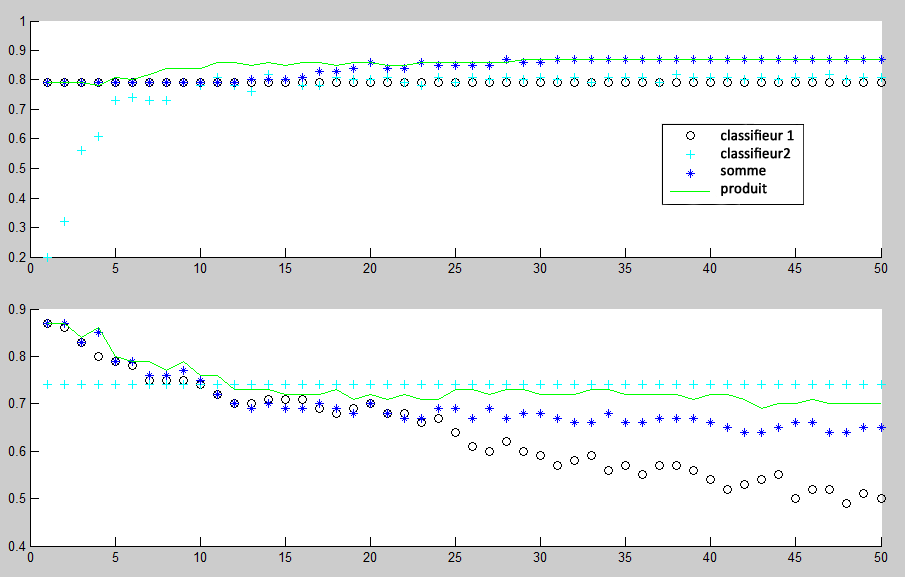
\includegraphics[width=\textwidth]{img/40-rates-function-of-d-k.png}
	\end{center}
	\caption{Variation des quatre taux de reconnaissance obtenus en fonction des paramètres $d$ (en haut) et $k$ (en bas)}
	\label{fig:ratecomparison}
\end{figure}

Globalement on observe de meilleurs résultats pour les combinaisons de classifieurs, représentés dans sur la figure ci-dessus en vert et en bleu foncé. Cependant, si l'on utilise les paramètres optimaux définis précédemment, les résultats sont biaisés : étant donné le paramètre $k$ fixé à 1, les probabilités résultant du second classifieur sont binaire, ce qui annule les résultats du premier classifieur dans le cas du produit mais aussi de la somme.